\chapter{Project 2: NAND gate}  \label{ch:nand}
Once one grasp the basic procedure to program an FPGA, by natural extension it should be asked how it is possible to exploit the full power of the SoM. This chapter offers a good start point, but it is just the tip of the iceberg. 
 



\section{Vivado project}
The project itself isn't changed: there is always the NAND gate. The only thing that is further added is the ability to boot the KR260 starter kit and to connect to it through the J-TAG interface. However, easy as it may seem, the procedure to follow is quite delicate and there are a lot of things to be taken care of.  The project will further analyze two ways of programming the FPGA: a) from within the SoM OS and b) at the boot of the board.
\begin{figure}[ht]
	\centering
	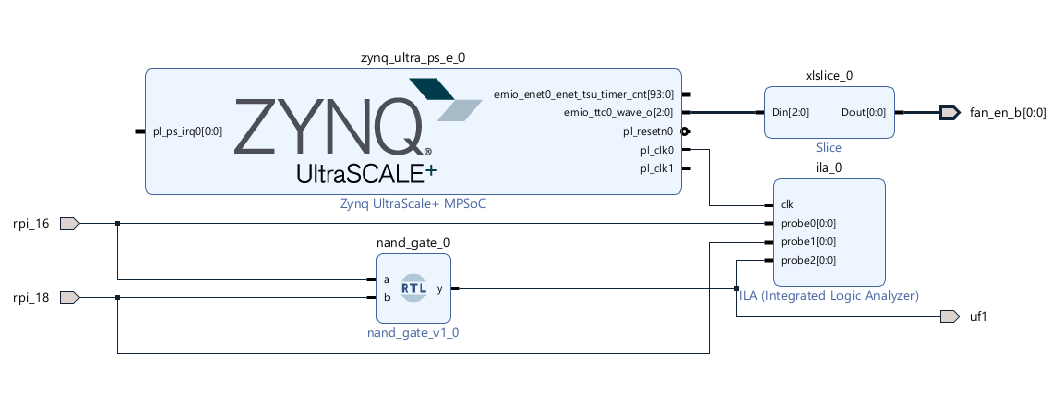
\includegraphics[width=\textwidth]{images/prj2_1}
	\caption{NAND gate Vivado block design.}
	\label{fig:prj2_1}
\end{figure}
Apart from the NAND design blobk, the project has been created from an example project given by AMD (this will include both the Zynq UltraScale+ MPsoC and the Slice). The ILA (Integrated Logic Analyzer) block serves the purpose to allow the view of the interesting waveform of the implementation during the debugging.
\bigskip
\\To create the project, open the Vivado main page, click on \textbf{Open Example Project} $\rightarrow$ \textbf{Next} $\rightarrow$ \textbf{Kria Starter Kit Design Example} $\rightarrow$ select the KR260 board $\rightarrow$ rename the project $\rightarrow$ \textbf{Default Bitstream} $\rightarrow$ create the project. To include both the source code of the NAND, follow the procedure explained in the previous chapter. The constrain file already exist, but it needs to be modified, adding the lines of code of the precious file. Once it is done, the file should look like in the following.
\begin{verbatim}
set_property BITSTREAM.GENERAL.COMPRESS TRUE [current_design]

#Fan Speed Enable
set_property PACKAGE_PIN A12 [get_ports {fan_en_b}]
set_property IOSTANDARD LVCMOS33 [get_ports {fan_en_b}]
set_property SLEW SLOW [get_ports {fan_en_b}]
set_property DRIVE 4 [get_ports {fan_en_b}]

#User defined pins
set_property PACKAGE_PIN F8 [get_ports {uf1}]
set_property IOSTANDARD LVCMOS18 [get_ports {uf1}]

set_property PACKAGE_PIN AA12 [get_ports {rpi_16}]
set_property IOSTANDARD LVCMOS33 [get_ports {rpi_16}]

set_property PACKAGE_PIN Y9 [get_ports {rpi_18}]
set_property IOSTANDARD LVCMOS33 [get_ports {rpi_18}]
\end{verbatim}
Open the design under the \textbf{IP INEGRATOR} section, add the NAND and the ILA blocks and connect them as it is showed in Figure \ref{fig:prj2_1}. Run both \textbf{Connection Automation} and \textbf{Block Automation} and let Vivado manage all the other connection. If needed, remake the wanted connections. Now, following the same procedure defined earlier, connect the I/O pins to the physical pins. The project should now be ready. 
To generate the wrapper, save the design and click on \textbf{Create HDL wrapper}. Make the new wrapper the top file (right click on the wrapper just created $\rightarrow$ \textbf{Make Top File}), generate the bistream, then move to \textbf{File} $\rightarrow$ \textbf{Export} $\rightarrow$ \textbf{Export Hardware} $\rightarrow$ \textbf{Include Bitstream}. The project is all set and it is now possible to focus on the Petalinux part.




\section{Petalinux project}
From within the Petalinux installation folder, type
\begin{verbatim}
	source ./settings.sh
\end{verbatim}
so as to set the Petalinux environment. Create now the project with the command
\begin{verbatim}
	petalinux-create --type project -s <path_to_bsp_file> --name <project_name>
\end{verbatim}
and once it is done, move into the folder just created. The following two steps are quite important, so it is recommended a bit more of attention.


\subsection{Base configuration}
The first configuration procedure aims to configure the core of the OS, i.e. to which architecture is addressed and which features are to be enabled. With the command
\begin{verbatim}
	petalinux-config --get-hw-description <path_to_xsa_file>
\end{verbatim}
a menu window will open (see Figure \ref{fig:prj2_2}), from which, moving into the various directories, the following packages must be enabled (or disabled):
\begin{itemize}
	\item \textbf{FPGA Manager} $\rightarrow$ \textbf{[*]FPGA Manager}
	\item \textbf{Image Packing Configuration} $\rightarrow$ \textbf{[]Copy final images to tftpboot}
\end{itemize}
\begin{figure}[ht]
	\centering
	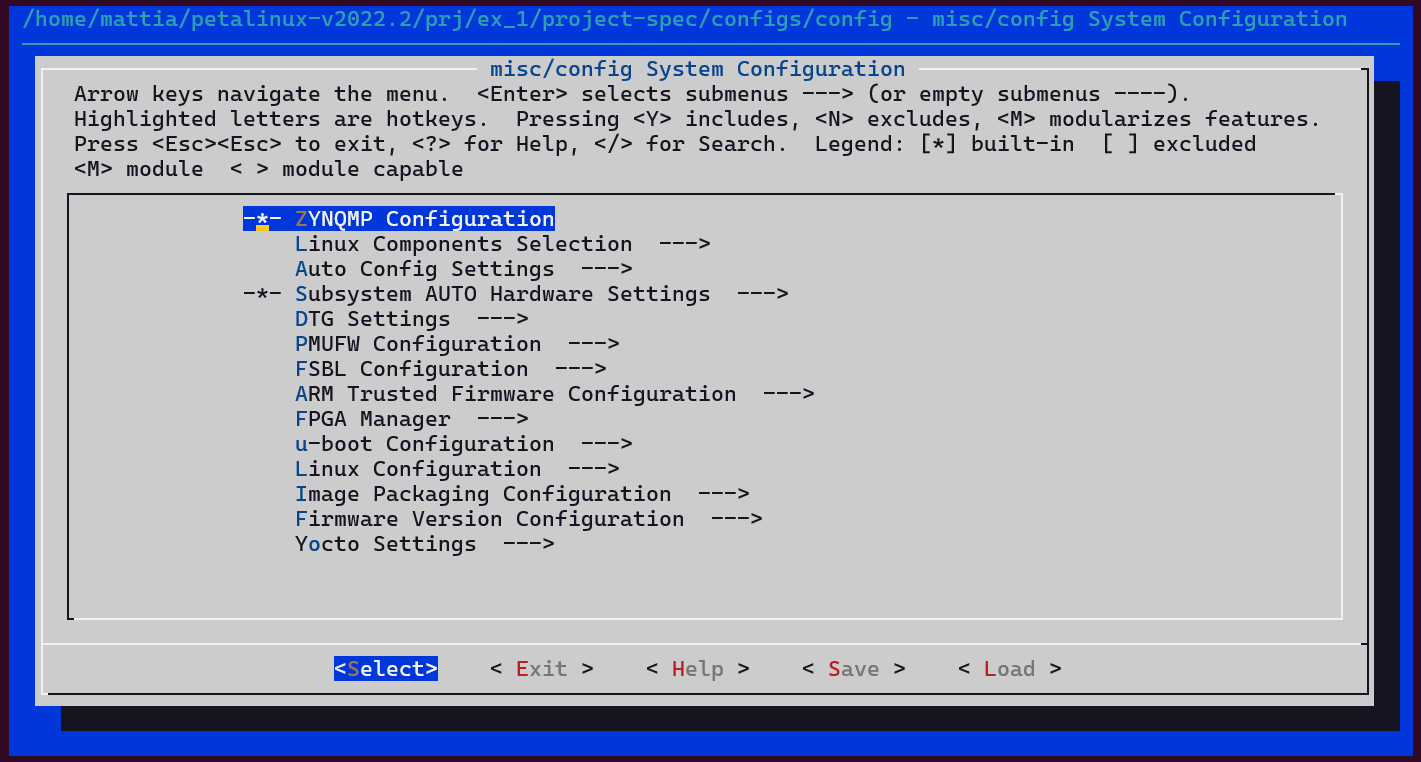
\includegraphics[width=\textwidth]{images/prj2_2}
	\caption{Base configuration window.}
	\label{fig:prj2_2}
\end{figure}
The FPGA manager will allow the FPGA to be programmed even during the operation of the board with few commands. However, it will generate an warning message during the creation of the BOOT.bin file.


\subsection{rootfs configuration}
The system to be created, in order to work, has to have some packages included, such as \textbf{bootget}, \textbf{gcc}, \textbf{XRT} and acceleration. The installation menu will open with the command
\begin{verbatim}
	petalinux-config -c rootfs
\end{verbatim}
from which the following packages have to be installed:
\begin{itemize}
	\item \textbf{Filesystem Packages} $\rightarrow$ \textbf{console} $\rightarrow$ \textbf{utils} $\rightarrow$ \textbf{git} $\rightarrow$ \textbf{[*]git}
	
	\item \textbf{Filesystem Packages} $\rightarrow$ \textbf{base} $\rightarrow$ \textbf{dnf} $\rightarrow$ \textbf{[*]dnf}
	
	\item \textbf{Filesystem Packages} $\rightarrow$ \textbf{x11} $\rightarrow$ \textbf{base} $\rightarrow$ \textbf{libdrm} $\rightarrow$ \textbf{[*]libdrm}, \textbf{[*]libdrm-tests}, \textbf{[*]libdrm-kms}
	
	\item \textbf{Filesystem Packages} $\rightarrow$ \textbf{libs} $\rightarrow$ \textbf{xrt} $\rightarrow$ \textbf{[*]xrt}, \textbf{[*]xrt-dev}
	
	\item \textbf{Filesystem Packages} $\rightarrow$ \textbf{libs} $\rightarrow$ \textbf{zocl} $\rightarrow$ \textbf{[*]zocl}
	
	\item \textbf{Filesystem Packages} $\rightarrow$ \textbf{libs} $\rightarrow$ \textbf{opencl-headers} $\rightarrow$ \textbf{[*]opencl-headers}
	
	\item \textbf{Filesystem Packages} $\rightarrow$ \textbf{libs} $\rightarrow$ \textbf{opencl-clhpp} $\rightarrow$ \textbf{[*]opencl-clhpp},\\ \textbf{[*]opencl-clhpp-dev}
	
	\item \textbf{Filesystem Packages} $\rightarrow$ \textbf{bootgen} $\rightarrow$ \textbf{[*]bootgen}, \textbf{[*]bootgen-dev}
	
	\item \textbf{Filesystem Packages} $\rightarrow$ \textbf{misc} $\rightarrow$ \textbf{packagegroup-core-buildessential} $\rightarrow$\\ \textbf{[*]packagegroup-core-buildessential},\\ \textbf{[*]packagegroup-core-buildessential-dev}
	
	\item \textbf{Filesystem Packages} $\rightarrow$ \textbf{misc} $\rightarrow$ \textbf{gcc-runtime} $\rightarrow$ \textbf{[*]libstdc++}, \\ \textbf{[*]libstdc++-dev}
	
	\item \textbf{Filesystem Packages} $\rightarrow$ \textbf{misc} $\rightarrow$ \textbf{gcr} $\rightarrow$ \textbf{[*]gcr}, \textbf{[*]gcr-dev}
	
	\item \textbf{Filesystem Packages} $\rightarrow$ \textbf{misc} $\rightarrow$ \textbf{gcr} $\rightarrow$ \textbf{[*]gdb}, \textbf{[*]gdb-dev}
	
	\item \textbf{Filesystem Packages} $\rightarrow$ \textbf{misc} $\rightarrow$ \textbf{glib-2.0} $\rightarrow$ \textbf{[*]glib-2.0}, \textbf{[*]glib-2.0-dev}
	
	\item \textbf{Filesystem Packages} $\rightarrow$ \textbf{misc} $\rightarrow$ \textbf{glibc} $\rightarrow$ \textbf{[*]glibc}, \textbf{[*]glibc-dev}, \textbf{[*]ldd}
	
	\item \textbf{Petaliunx Package Groups} $\rightarrow$ \textbf{packagegroup-petalinux} $\rightarrow$ \\ \textbf{[*]packagegroup-petalinux}
	
	\item \textbf{Petaliunx Package Groups} $\rightarrow$ \textbf{packagegroup-petalinux-gstreamer} $\rightarrow$\\ \textbf{[*]packagegroup-petalinux-gstreamer}
	
	\item \textbf{Petaliunx Package Groups} $\rightarrow$ \textbf{packagegroup-petalinux-opencv} $\rightarrow$\\ \textbf{[*]packagegroup-petalinux-opencv}
	
	\item \textbf{Petaliunx Package Groups} $\rightarrow$ \textbf{packagegroup-petalinux-v4lutils} $\rightarrow$\\ \textbf{[*]packagegroup-petalinux-v4lutils}
	
	\item \textbf{Petaliunx Package Groups} $\rightarrow$ \textbf{packagegroup-petalinux-x11} $\rightarrow$\\ \textbf{[*]packagegroup-petalinux-x11}
\end{itemize}
After this boring procedure, it is time to build the project with the command
\begin{verbatim}
	petalinux-build
\end{verbatim}
In the case of building failure with error messages not related to the implementation, try to clear out the current files by typing
\begin{verbatim}
	petalinux-config -x mr proper
\end{verbatim}
command which is used to deep cleaning the workspace, similar to how it's used in the Linux kernel build system.
\begin{figure}[ht]
	\centering
	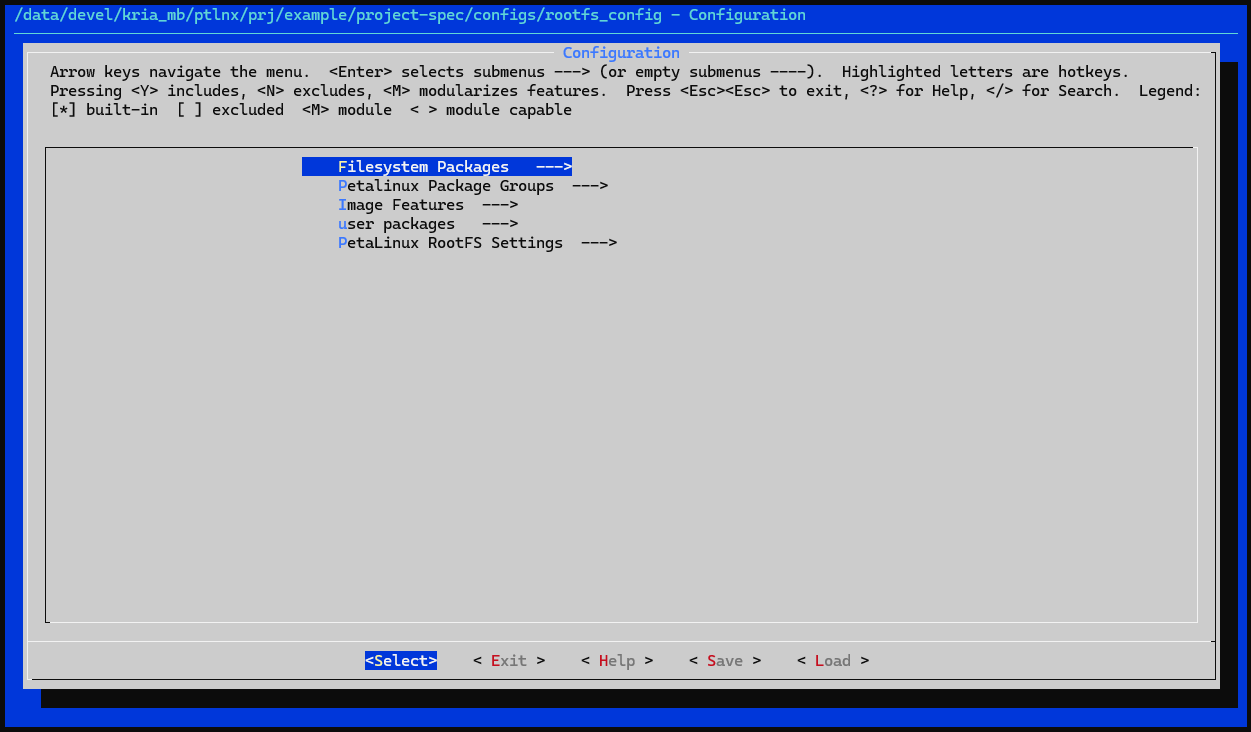
\includegraphics[width=\textwidth]{images/prj2_3}
	\caption{rootfs configuration window.}
	\label{fig:prj2_3}
\end{figure}


\subsection{Booting the board}
Since the board boots from a SD card, the system configuration just created has to be converted into a bootable image for the card. First step to carry out is the creation of the BOOT.bin file, which is of quite importance. To do so, after the project build, the command line is (on the same line)
\begin{verbatim}
	petalinux-package --boot --fsbl <path_to_elf_file> --fpga <path_to_bitstream>
	--u-boot
\end{verbatim}
in which the .elf file is usually located under the path images/linux/. The second step is to create a .wic image for the SD card to be flashed in. The command to do that is (on the same line)
\begin{verbatim}
	petalinux-package --wic --images-dir images/linux/ --bootfiles
	"ramdisk.cpio.gz.u-boot,boot.scr,Image,system.dtb,system-zynqmp-sck-kr-g
	-revB.dtb" --disk-name "sda"
\end{verbatim}
from which the .wic image will be generated and found in the same folder as the .elf file. To flash the SD card make use of a third-part software, such as balenaEtcher or something similar. Once the flash is done, insert the SD in the board and power it up. With a third part software, such as PuTTY, connect to the serial port (Baud Rate 115200). The system will require to inset some credential and the following may be used:
\begin{verbatim}
	ligin : petalinux
	password : your_password
\end{verbatim}
and now everything is set. To check if the packages are actually installed, type in the serial terminal
\begin{verbatim}
	gcc --version
	bootgen
\end{verbatim}
and some messages relating to the version or how to use them will be displayed.




\section{Programming the FPGA}
So far, only the boot was done with the procedure defined. The FPGA is not actually programmed. To do so, two ways can be used: the On-Run programming and the Boot programming. The first one allows for more flexibility and has the advantage to let the FPGA to be programmed even when the system is running, without the need to repeat all the steps previously explained. The second, thought being more rigid, allows for the FPGA to be programmed each time the system boots up. Within this example, the first approach has been chosen. To actually program the FPGA in after the system is booted, there is the need to convert the bitstream into a .bin file and then "manually" load it into the FPGA through the FPGA manager. Both .bit and the .bif file are to be copied in the SD card into an accessible folder. The .bif file has the following command lines:
\begin{verbatim}
	all:
	{
	    bit_file_name.bit
	}
\end{verbatim}
and through that the .bin file can be created using the command
\begin{verbatim}
	sudo bootgen -image <bif_file> -arch zynqmp -process_bitstream bin
\end{verbatim}
Now the .bin file has to be copied into the folder at the /lib/firmware path. The last step to program the FPGA is to load the file with the command:
\begin{verbatim}
	sudo sh -c 'echo "bin_file" > /sys/class/fpga_manager/fpga0/firmware'
\end{verbatim}





\section{J-TAG debugging}
Vivado offers a very valid way to debug the program just created. This is made possible thanks to the ILA (Integrated Logic Analyzer), which "reads" the internal signals to which its probes are connected, save them to a RAM BUS and the, through J-TAG, they can be seen in a similar way an oscilloscope plots the red signals. Actually, its functioning it very similar to an oscilloscope itself.
\bigskip
\\Once the FPGA is programmed, open Vivado's \textbf{Hardware Manager} and repeat the same connecting procedure as for the bare programming. After the successful connection, in the Hardware window, under the FPGA's name, the ILA hw will appear. Double click on it and in the main window will be displayed all the selected signals alongside with their waveform. In the \textbf{Trigger Set Up} window, chose the triggering signal and triggering condition and then click on the \text{Play} button of the main window. 
\bigskip
\\For this project, the debugging may be less interesting than effectively seeing the board's led turn on and off according to the NAND's truth table. However, knowing how to set up the debugging is quite useful, especially for future, more complex applications. In the following chapter a more debug-reliable example is explained.